\documentclass{article}
\usepackage[spanish]{babel}
\usepackage[utf8]{inputenc}
\usepackage{graphicx}
\usepackage[outdir=./]{epstopdf}
\usepackage{subfigure}
\usepackage{amsmath}
\usepackage{amsfonts}
\usepackage{algorithm}
\usepackage{algorithmic}
\floatname{algorithm}{Algoritmo}
\renewcommand{\listalgorithmname}{Lista de algoritmos}
\renewcommand{\algorithmicrequire}{\textbf{Entrada:}}
\renewcommand{\algorithmicensure}{\textbf{Salida:}}
\renewcommand{\algorithmicend}{\textbf{fin}}
\renewcommand{\algorithmicif}{\textbf{si}}
\renewcommand{\algorithmicthen}{\textbf{entonces}}
\renewcommand{\algorithmicelse}{\textbf{si no}}
\renewcommand{\algorithmicelsif}{\algorithmicelse,\ \algorithmicif}
\renewcommand{\algorithmicendif}{\algorithmicend\ \algorithmicif}
\renewcommand{\algorithmicfor}{\textbf{para}}
\renewcommand{\algorithmicforall}{\textbf{para todo}}
\renewcommand{\algorithmicdo}{\textbf{hacer}}
\renewcommand{\algorithmicendfor}{\algorithmicend\ \algorithmicfor}
\renewcommand{\algorithmicwhile}{\textbf{mientras}}
\renewcommand{\algorithmicendwhile}{\algorithmicend\ \algorithmicwhile}
\renewcommand{\algorithmicloop}{\textbf{repetir}}
\renewcommand{\algorithmicendloop}{\algorithmicend\ \algorithmicloop}
\renewcommand{\algorithmicrepeat}{\textbf{repetir}}
\renewcommand{\algorithmicuntil}{\textbf{hasta que}}
\renewcommand{\algorithmicprint}{\textbf{imprimir}} 
\renewcommand{\algorithmicreturn}{\textbf{devolver}} 
\renewcommand{\algorithmictrue}{\textbf{cierto }} 
\renewcommand{\algorithmicfalse}{\textbf{falso }} 


\title{
\includegraphics[width=\columnwidth]{resources/images/cinvestav-header}\\PCA\\Principal Component Analysis}
\author{Rafael Pérez Torres\\Tópicos selectos en reconocimiento de patrones\\Profesor: Dr. Wilfrido Gómez}
\date{3 julio 2015}
\begin{document}
\maketitle

\begin{abstract}
El presente documento presenta una introducción a las técnicas de reducción de dimensionalidad, describiendo tópicos como la maldición de la dimensionalidad así como una clasificación general de las técnicas de reducción.
Específicamente, se describe el Análisis de Componentes Principales (PCA) como una técnica no paramétrica para la reducción de dimensionalidad, presentando su fundamento matemático y el método de descomposición de eigenvalores como mecanismo para selección de los componentes principales.
\end{abstract}

\section{Introducción}

\paragraph{La maldición de la dimensionalidad}
\label{par:la_maldicion_de_la_dimensionalidad}
La maldición de la dimensionalidad es un término acuñado por Bellman en 1961, y se refiere al hecho de que el tamaño de la muestra para estimar una función de varias \emph{variables} con un grado específico de precisión aumenta exponencialmente con el número de variables.

\paragraph{El fenómeno del espacio vacío}
\label{par:el_fenomeno_del_espacio_vacio}
Acuñado por Scott y Thompson, el fenómeno del espacio vacío es responsable de la maldición de la dimensionalidad, indicando que los espacios de altas dimensiones son inherentemente dispersos (\emph{sparse}).

\paragraph{Dimensión intrínseca}
\label{par:dimension_intrinseca}
La dimensión intrínseca de un fenómeno es el número de variables independientes que explican o describen de forma satisfactoria a dicho fenómeno.
A partir de ella se puede realizar la reducción de dimensionalidad sin caer en casos extremos.

\paragraph{Reducción de la dimensionalidad}
\label{par:reduccion_de_la_dimensionalidad}
Dada una cantidad de características, ¿Cómo pueden seleccionarse las más importantes de forma que se reduzca su cantidad y al mismo tiempo se conserve la mayor cantidad de información discriminatoria posible?

\paragraph{¿Por qué es posible reducir la dimensionalidad?} 
\label{par:por_que_es_posible_reducir_la_dimensionalidad}
A menudo, la representación de los datos será posible por distintos motivos:
\begin{itemize}
	\item Muchas de las variables son menores que el tamaño del ruido por lo que son irrelevantes.
	\item Muchas de las variables están correlacionadas con otras.
\end{itemize}

\paragraph{Tipos de reducción de dimensionalidad}
\label{par:tipos_de_reduccion_de_dimensionalidad}
Existen dos mecanismos principales para reducir la cantidad de variables en un sistema (Figura~\ref{fig:reduccion-dimensionalidad}):
\begin{itemize}
	\item \textbf{Extracción-Generación de características}: Dado un espacio de características $\mathbf{x}_i \in \mathbb{R} ^M$, encontrar un mapeo $\mathbf{y} = f(x):\mathbb{R}^M \to \mathbb{R}^m$, con $m<M$, tal que el vector transformado $\mathbf{y}_i \in \mathbb{R}^m$ preserve la información en $\mathbb{R}^M$.
	\item \textbf{Selección de características}: Dado un espacio de características $\mathbf{x}_i = \left \{ x_j | j = 1, \ldots, M  \right \}$ encontrar un subconjunto $\mathbf{y}_i=\left \{x_{i1},\ldots,x_{im} \right \}$, con $m<M$, tal que se maximice el desempeño de la clasificación.
\end{itemize}

\begin{figure}
	\centering
	\subfigure[Generación de características]{
		%\label{fig:generacion-caracteristicas}
		$	
		\begin{bmatrix}
			x_1\\ 
			x_2\\ 
			\vdots\\ 
			x_M\\ 
			\end{bmatrix}
			\to
			\begin{bmatrix}
			y_1\\ 
			y_2\\ 
			\vdots\\ 
			y_M\\ 
			\end{bmatrix}
			=f \left (
			\begin{bmatrix}
			x_1\\ 
			x_2\\ 
			\vdots\\ 
			x_3\\ 
			\end{bmatrix}
			\right ) 
		$
	}

	\subfigure[Selección de características]{
	$
	\begin{bmatrix}
	x_1\\ 
	x_2\\ 
	\vdots\\ 
	x_M\\ 
	\end{bmatrix}
	\to
	\begin{bmatrix}
	x_{i1}\\ 
	x_{i2}\\ 
	\vdots\\ 
	x_{iM}\\ 
	\end{bmatrix}
	$
	}
	\caption{Reducción de dimensionalidad}
	\label{fig:reduccion-dimensionalidad}
\end{figure}

\section{Principal Component Analysis PCA} 
\label{sec:principal_component_analysis_pca}
El Análisis de Componentes Principales es una herramienta estándar en el análisis de datos moderno debido a que es no paramétrico, es simple, y existen algoritmos relativamente eficientes para su cálculo.

En términos simples, la técnica PCA busca identificar las bases más significativas para reexpresar un conjunto de datos que filtre el ruido y revele estructuras ocultas.

\subsection{Caso de uso básico}
\label{sub:ejemplo_basico}
Considérese que se desea estudiar el movimiento de un resorte ideal.
Asumiendo que se ignoran conocimientos de física, se prepara un dispositivo experimental que consiste en el resorte y tres cámaras de video colocadas en posiciones arbitrarias $(\overrightarrow{a},\overrightarrow{b},\overrightarrow{c})$, como se muestra en la Figura~\ref{fig:resorte}.
\begin{figure}
	\centering
	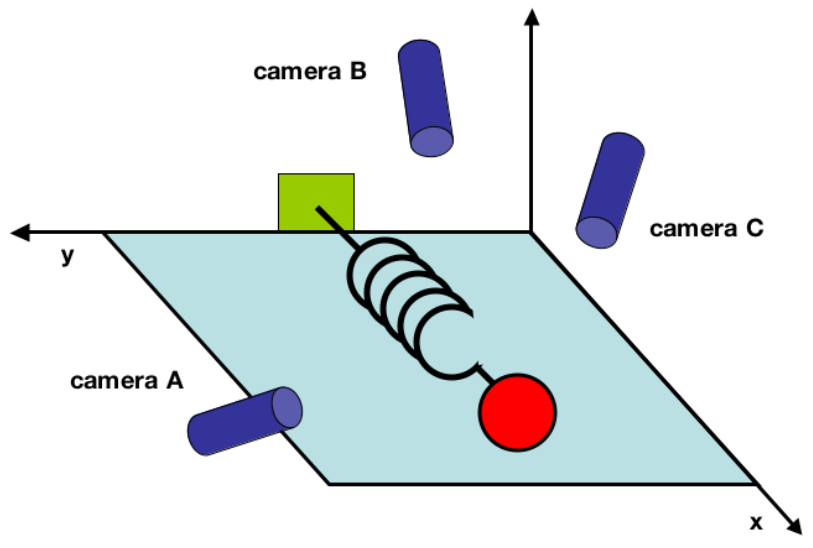
\includegraphics[scale=0.35]{resources/images/resorte}
	\caption{Sistema para estimación del comportamiento de un resorte}
	\label{fig:resorte}
\end{figure}

Intuitivamente sabemos que el movimiento se concentra únicamente en el eje $X$, pero ¿Cómo pasar de lo detectado por las cámaras en la Figura~\ref{fig:camaras} hacia esto?
\begin{figure}
	\centering
	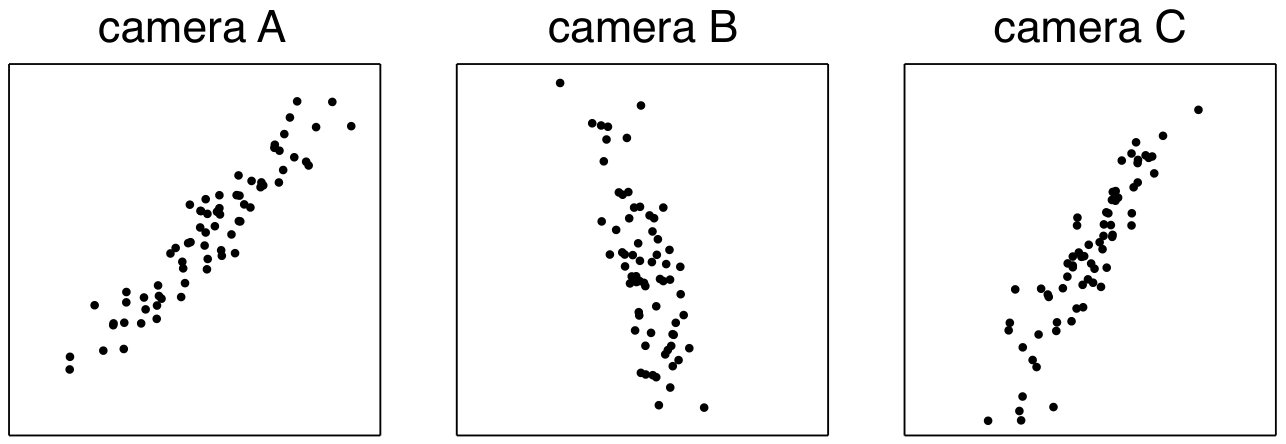
\includegraphics[width=\columnwidth]{resources/images/camaras}
	\caption{Datos obtenidos por las cámaras}
	\label{fig:camaras}
\end{figure}


En el mundo real, típicamente se trabaja \emph{a ciegas} y no es posible conocer con anticipación la mejor posición en la que las \emph{cámaras} deban ser colocadas.

\subsection{Fundamentos matemáticos del PCA}
\label{sub:fundamentos_matematicos_del_pca}
PCA asume que los datos puedes ser representados como una combinación lineal de sus vectores básicos (Figura \ref{fig:combinacion-lineal}).

\begin{figure}
	\centering
	$v = k_1v_1 + k_2v_2 + \ldots + k_nv_n = \sum_{i=1}^n k_iv_i$
	\caption{Ejemplo de combinación lineal}
	\label{fig:combinacion-lineal}
\end{figure}

Sea $\mathbf{X}$ una matriz $m \times n$ el conjunto original de datos, $\mathbf{Y}$ otra matriz $m \times n$ que almacenará la nueva representación de los datos realizada a través de una transformación lineal con la matriz $\mathbf{P}$.
Entonces se tiene:
\begin{equation}
\mathbf{PX} = \mathbf{Y}
\label{eq:ecuacion-inicial}
\end{equation}
A partir de~\ref{eq:ecuacion-inicial} es posible interpretar que:
\begin{itemize}
	\item Geométricamente, $P$ es una rotación y estrechamiento que transforma a $\mathbf{X}$ en $\mathbf{Y}$
	\item Las filas de $\mathbf{P}$, $\left \{ p_1,\ldots,p_m \right \}$ son el nuevo conjunto de vectores base para expresar a los elementos de $\mathbf{X}$, como se muestra en la Figura~\ref{fig:vectores-base}.
	\item El $j$-ésimo coeficiente de $y_i$ es una proyección sobre la $j$-ésima fila de $\mathbf{P}$
\end{itemize}

\begin{figure}
	\centering
	\subfigure[]{
		$
		\mathbf{PX} =
\begin{bmatrix}
p_1 \\ \vdots \\ p_m
\end{bmatrix}
\begin{bmatrix}
x_1 & \cdots & x_n
\end{bmatrix}
		$
	}
	\subfigure[]{
	$
	Y =
\begin{bmatrix}
p_1x_1 & \ldots & p_1x_n\\ 
\vdots & \ddots & \vdots \\ 
p_mx_1 & \cdots & p_mx_n
\\ 

\end{bmatrix}
	$
	}
	\caption{Nuevos vectores base}
	\label{fig:vectores-base}
\end{figure}

De lo anterior se desprende que los vectores fila $\left \{ p_1,\ldots,p_m \right \}$ en $\mathbf{P}$ serán los componentes principales de $\mathbf{X}$.
Para encontrar la mejor forma para reexpresar $\mathbf{X}$ así como una buena elección para $\mathbf{P}$ es necesario identificar las características que nos gustaría que $\mathbf{Y}$ exhiba.

\paragraph{Elementos para describir los datos} 
\label{par:elementos_para_describir_los_datos}
\subparagraph{Ruido y rotación} 
\label{subp:ruido_y_rotacion}
El nivel del ruido en cualquier conjunto de datos debería ser bajo.
No existe una escala absoluta para su medición pero sí para obtener una referencia cuantitativa respecto a la magnitud de la \emph{señal} descrita por los datos.
Una métrica común es el radio señal a ruido (SNR), o un radio de varianzas $\sigma^2$,
$$
SNR = \frac{\sigma^2_{\text{signal}}}{\sigma^2_{\text{noise}}}
$$

Un valor de SNR alto ($>1$) indica una medición de alta precisión, mientras que un valor bajo indica datos muy ruidosos.
Esta relación es mostrada en la Figura~\ref{fig:snr-varianza}, donde puede apreciarse que la dirección de mayor varianza coincide con el eje mayor de la nube de puntos; así se infiere que la dinámica de interés ocurre en la dirección con la mayor varianza y presumiblemente el más alto valor de SNR.
\begin{figure}
	\centering
	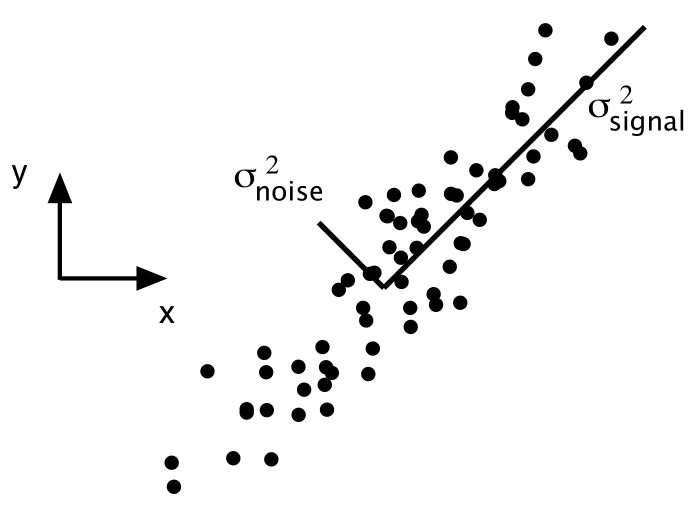
\includegraphics[scale=0.35]{resources/images/snr}
	\caption{Relación entre SNR y varianza de los datos}
	\label{fig:snr-varianza}
\end{figure}


\subparagraph{Redundancia}
\label{subp:redundancia}
La redundancia entre características ocurre cuando a partir del valor de un atributo $r1$ es posible calcular el valor de un atributo $r2$.
La Figura~\ref{fig:redundancia} muestra diferentes niveles de redundancia entre dos atributos.
Idealmente, se busca considerar la menor cantidad de variables, por lo que aquellas redundantes son discriminadas.
\begin{figure}
	\centering
	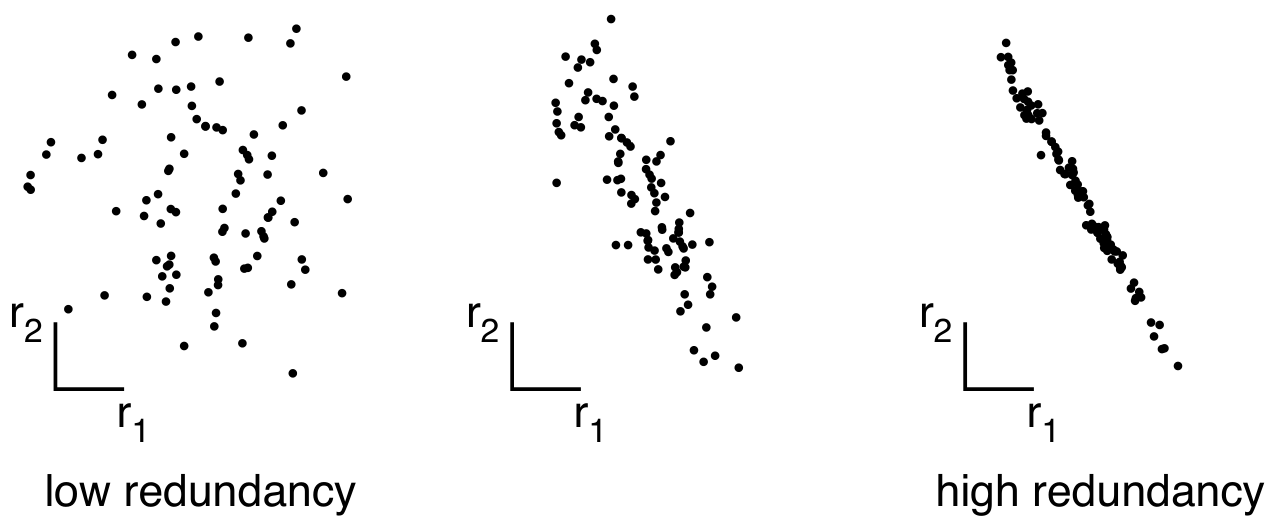
\includegraphics[width=\columnwidth]{resources/images/redundancia}
	\caption{Niveles de redundancia}
	\label{fig:redundancia}
\end{figure}

\subparagraph{Matriz de covarianza}
\label{subp:matriz_de_covarianza}
La covarianza permite conocer el grado de relación lineal entre dos variables.
Un gran valor positivo indica correlación positiva, mientras que un gran valor negativo denota correlación negativa.
Por consiguiente, el valor absoluto de la covarianza mide el grado de redundancia.
Si cada fila de $\mathbf{X}$ representa todas las mediciones de un tipo, cada columna corresponde al conjunto de medidas tomadas en una lectura en particular:
$$
\mathbf{X} = 
\begin{bmatrix}
x_1 \\
\vdots \\
x_m
\end{bmatrix}
$$
entonces la matriz de covarianza $mathbf{C_X}$ puede ser expresada como:
$$
C_X \equiv \frac{1}{n}\mathbf{XX}^T
$$
donde el $ij$-ésimo elemento de $\mathbf{C_X}$ corresponde al producto punto entre el vector $i$-ésimo y el vector $j$-ésimo de $\mathbf{X}$.
La matriz $\mathbf{C_X}$ es cuadrada de tamaño $m \times m$ además de simétrica y permite conocer los valores de ruido y redundancia de los datos sabiendo que:
\begin{itemize}
	\item Su diagonal incluye la varianza de cada característica, valores grandes indican importancia estructural.
	\item Los elementos no diagonales definen la covarianza entre cada par de atributos, valores grandes indican alta redundancia.
\end{itemize}

De esta manera, en la nueva matriz de covarianza $\mathbf{C_Y}$ se desea contener los datos reestructurados intentando a) minimzar redundancia (medida mediante la covarianza) y b) maximizar la señal (medida mediante la varianza).
Por ello, la matriz $\mathbf{C_Y}$ debería tener la siguiente estructura:
\begin{itemize}
	\item Los elementos no diagonales deberían ser 0, convirtiéndola en una matriz diagonal que es \emph{de-correlacionada}.
	\item Cada dimensión en $\mathbf{Y}$ debería ser ordenada de acuerdo a su varianza.
\end{itemize}

El elemento restante de la ecuación inicial~\ref{eq:ecuacion-inicial} es $\mathbf{P}$ quien se comporta como una rotación para alinear los datos con el eje de máxima varianza.
La idea general de su cálculo es mostrada en el Algoritmo~\ref{alg:algoritmo-solucion-p}.

\begin{algorithm} 
\begin{algorithmic}[1] 
\STATE Seleccionar una dirección en el espacio $m$-dimensional en el que la varianza de $\mathbf{X}$ es maximizada y guardar dicho vector como $\mathbf{p_1}$.
\STATE Encontrar otra dirección donde la varianza sea maximizada, restringiendo la búsqueda a las direcciones ortogonales a todas las direcciones previamente seleccionadas. Almacenar este nuevo vector como $\mathbf{p_i}$.
\STATE Repetir el procedimiento hasta que $m$ vectores hayan sido seleccionados.
\end{algorithmic} 
\caption{Algoritmo para encontrar el valor de $\mathbf{P}$} 
\label{alg:algoritmo-solucion-p}
\end{algorithm}

Al ordenar el conjunto resultante en $\mathbf{p}$ se obtienen los componentes principales.

\section{Solución de PCA a través de descomposición de eigenvectores}
\label{sec:solucion_de_pca_a_traves_de_eigenvectores}
El objetivo de la solución es encontrar una matriz ortonormal $\mathbf{P}$ en $\mathbf{Y} = \mathbf{PX}$ tal que $\mathbf{C_Y} \equiv \frac{1}{n}\mathbf{YY}^T$.
Las filas de $\mathbf{P}$ son los componentes principales de $\mathbf{X}$.

Expresando $\mathbf{C_Y}$ en términos de la variable desconocida $\mathbf{P}$:
\begin{eqnarray}
\mathbf{C_Y} 	&=& \frac{1}{n} \mathbf{YY}^T \\
				&=& \frac{1}{n} (\mathbf{PX})(\mathbf{PX})^T \\
				&=& \frac{1}{n} \mathbf{PXX}^T\mathbf{P}^T \\
				&=& P(\frac{1}{n} \mathbf{XX}^T)\mathbf{P}^T \\
\mathbf{C_Y}	&=& \mathbf{PC_XP}^T
\end{eqnarray}

Cualquier matriz simétrica $\mathbf{A}$ es diagonalizada por una matriz ortogonal\footnote{Una matriz $A$ es ortogonal si $AA^T = \mathbb{I}$} de sus eigenvectores, esto es $\mathbf{A}=\mathbf{EDE}^T$.
Al seleccionar que la matriz $\mathbf{P}$ sea una matriz donde cada renglón $\mathbf{p_i}$ es un eigenvector de $\frac{1}{n}\mathbf{XX}^T$, se logra que $\mathbf{P} \equiv \mathbf{E^T}$.
Adicionalmente se debe considerar que $\mathbf{P^{-1} = P^T}$
Utilizando estos elementos, es posible terminar de evaluar $\mathbf{C_Y}$ como:
\begin{eqnarray}
\mathbf{C_Y}	&=& \mathbf{PC_XP}^T \\
				&=& \mathbf{P(E^TDE)P^T} \\
				&=& \mathbf{P(P^TDP)P^T} \\
				&=& \mathbf{(PP^T)D(PP^T)} \\
				&=& \mathbf{(PP^{-1})D(PP^{-1})} = \mathbf{\mathbb{I}D\mathbb{I}}\\
\mathbf{C_Y}	&=& \mathbf{D}
\end{eqnarray}
donde puede apreciarse que la elección de $\mathbf{P}$ diagonaliza a $\mathbf{C_Y}$.
Dentro de $\mathbf{P}$ y $\mathbf{C_Y}$ se encuentran los resultados de PCA:
\begin{itemize}
	\item Los componentes principales son los eigenvectores de $\mathbf{C_X} = \frac{1}{n}\mathbf{XX}^T$.
	\item El $i$-ésimo valor diagonal de $\mathbf{C_Y}$ es la varianza de $\mathbf{X}$ a lo largo de $\mathbf{p_i}$
\end{itemize}

Los pasos para encontrar la solución a PCA para un conjunto de datos son mostrados en el Algoritmo~\ref{alg:algoritmo-pca-eigenvectores}.

\begin{algorithm} 
\begin{algorithmic}[1] 
\STATE Obtener y sustraer la media de los datos.
\STATE Calcular la matriz de covarianza $\Sigma$ .
\STATE Calcular los eigenvectores para $\Sigma$ .
\STATE Selección de componentes.
\STATE Formación del nuevo conjunto de datos.
\end{algorithmic} 
\caption{Algoritmo para PCA a través de eigenvectores} 
\label{alg:algoritmo-pca-eigenvectores}
\end{algorithm}

\subsection{Obtención y sustracción de la media de los datos}
\label{sub:obtencion_y_sustraccion_de_la_media_de_los_datos}
Se debe obtener la media y sustraerla a los datos por cada dimensión.
Esta diferencia es utilizada para calcular la matriz de covarianza.
$$
\mu = \sum_{i=1}^n x_i - \overline{x} 
$$

\subsection{Cálculo de la matriz de covarianza} 
\label{sub:calculo_de_la_matriz_de_covarianza}
Como ha sido descrito, la matriz de covarianza permite medir la redundancia y varianza de los datos.
Es calculada a través de:
$$
\Sigma = \frac{\sum_{i=1}^n (x_i - \overline{x})(y_i - \overline{y})}{(n-1)}
$$

\subsection{Cálculo de eigenvectores}
\label{sub:calculo_de_eigenvectores}
El autovector, vector propio o eigenvector $\mathbf{v}$ de una matriz $\mathbf{M}$ de $(n \times n)$ es una matriz de ($n \times 1$) tal que al multiplicarse por un elemento $v$ obtiene un múltiplo de sí mismo.
Esto se expresa como $A\mathbf{v} = \lambda v$, donde $\lambda$ es un valor escalar real que recibe el nombre de autovalor, valor propio o eigenvalor.

A menudo, una transformación queda completamente determinada por sus vectores propios y valores propios.
Entonces, su importancia radica en que pueden explicar la transformación que PCA realiza para encontrar la nueva base de los datos.

La mayoría de las herramientas computacionales para análisis de datos cuentan con alguna implementación para obtener eigenvalores y eigenvectores.

\subsection{Selección de componentes}
\label{sub:seleccion_de_componentes}
Los eigenvectores con los valores más altos son los componentes principales del conjunto de datos. 
Por lo tanto, los eigenvectores habrán de ordenarse de forma descendente (considerando el eigenvalor asociado a cada uno de ellos) para obtener los componentes por orden de importancia.

Existen distintos mecanismos para decidir la cantidad de eigenvectores a seleccionar, algunos indican seleccionar aquellos que describan a los datos al menos en un porcentaje determinado, otros cuando la separación entre dos eigenvectores consecutivos es grande.

A partir de los $m$ eigenvectores seleccionados se forma la matriz de transformación $\mathbf{P}$:
$$
P = \left \{ \text{eig}_1,\text{eig}_2,\ldots,\text{eig}_m \right \}
$$


\subsection{Formación del nuevo conjunto de datos}
\label{sub:formacion_del_nuevo_conjunto_de_datos}
Una vez seleccionados los eigenvectores a considerar, se debe crear el nuevo conjunto de datos.
Esto es realizable a través de:
$$
\text{Datos finales} = \textbf{P}^T \textbf{X}
$$ 


\section{Conclusiones}
\label{sec:conclusiones}
Se ha presentado una introducción a la reducción de dimensionalidad y una clasificación de las técnicas relacionadas.
Asimismo, se ha presentado una descripción del fundamento matemático y comportamiento del PCA como herramienta no supervisada para la generación de las características más representativas de un conjunto de datos.

\end{document}

% http://www.cs.otago.ac.nz/cosc453/student_tutorials/principal_components.pdf